\documentclass{article}
\usepackage{blindtext}
\usepackage[utf8]{inputenc}
\usepackage{graphicx}
\usepackage{mathpazo}
\usepackage{amsmath, amsfonts}
\usepackage{float}
\usepackage[section]{placeins}
\usepackage{fancyvrb}
\usepackage[affil-it]{authblk} 
\usepackage{verbatim}
\usepackage[normalem]{ulem}

\pagenumbering{arabic}
\title{Math 381: Discrete Mathematical Modeling Final Project}
\author{Yanni Du, Tim Turner, Yuqi Huang, Evan Ko }
\affil{University of Washington}
\date{August 16 2017}
\begin{document}
	
\maketitle
\newpage
\tableofcontents
\newpage

\section{Abstract}

We wish to model and predict the price of a stock in thirty days after the last known prices, while understanding the risk of potentially suffering a loss. Geometric Brownian motion is used to predict the expected price per share of Apple's stock after thirty days. Three strategies are reviewed: using standard model, including beta parameter, and including random variables to induce varied shocks. Using Monte Carlo simulation we test the model and effect of adding additional parameters and variables. By making a prediction of a date in the past, we compare our model to the actual changes in stock price giving us a baseline to analyze accuracy of our prediction. We find the initial model normally predicts the price precisely to within a range of a few dollars when there are no unexpected events or market volatility. Additional results allow for useful risk analysis, describing the chance of a net decrease in price.

\section{Problem Description}
\subsection{Problem}
Is it possible to predict future price per share of a stock (e.g. Apple) 30 days after the last known price using that stock's historical data? If so, what are the chances of an inaccurate prediction or worse, suffering a net loss?

\subsection{Background}
Inherently, stock prices are \textit{not} known in advance or predictable with complete certainty, simply because any number of events can occur that might effect the price of a stock. The Random Walk Theory even suggests that stock price changes have the same distribution and are independent of each other, so the past movement or trend of a stock price or market cannot be used to predict its future movement.\cite{RW}\\
However, in the real world, this theory is never popular among investigators, especially when people have fast access to relevant news and resources nowadays. Even in cases where our prediction might not be accurate, we hope there will be precision in our results evidenced through proportional effect caused by different events.

\subsection{Questions}

Some questions we're looking to answer include
\begin{itemize}
	\item What equations provide the best elements for a model and why?
    \item What things affect stock? Events, stock age, company, time of day, etc
    \item What events might affect a stock?
    \item Which types of events are more likely to affect a stock?
    \item Can events be profiled with properties that show the magnitude of their impact on a stock?
    \item Do similar event profiles share similar probability distributions?
    \item How do multiple factors, each with their own unique effect, combine to affect stock?
\end{itemize}

\section{Simplifications and Modeling}
\subsection{Simplification and Assumptions}
In this project, we simplify the Brownian model of financial markets. The model has some original assumptions that we are also using: \cite{WikiBModel}
\begin{itemize}
	\item We assume a frictionless market that no transaction costs occur either for buying or selling.
    \item The asset has continuous prices evolving in time and are driven by Geometric Brownian Motion processes.
    \item There are no surprises in the market. 
\end{itemize}
In our project, instead of analyzing the price of a portfolio, which is the combination of investing in bond and stocks, we simplify the model by only analyzing one stock price, the stock price of Apple. We also add one more assumption that the stock does not pay a dividend.\\
With these simplifications, we are now focusing our project on a part of an investment instead of the whole portfolio. We still give a nice model showing how Monte Carlo simulation is used in finance. \\
Additionally, we are going to simulate the stock price based on Geometric Brownian Motion in this project instead of Brownian motion, which is used in the original model. Brownian motion is a continuous-time stochastic process. However, since Brownian motion takes negative values, it is questionable to model the stock price. On the contrary, Geometric Brownian Motion is the exponential of the Brownian Motion process, one of the reasons that geometric Brownian motion is used to model financial and other processes that cannot be negative.\cite{GBMoverBM} \\

\section{Mathematical Model}

\subsection{Model Adaptation for Monte Carlo}
In order to convert our simplified model into a mathematical model that can be solved using a Monte Carlo simulation we need to find or choose what values will be used for our parameters and how we will implement our randomness in the random variable component.\\
To this end, in our specific case we have for any given day $t \in \{1,2,...,30\}$ the next day's predicted stock price $S_{t+1}$ will close according to:

\begin{align*}
S_{t+1} = S_{t}exp\left [ \left ( \mu -\frac{\sigma ^{2}}{2} \right ) +\sigma \epsilon \right ] \\
\end{align*}

Constant Drift component: $\mu - \frac{\sigma ^{2}}{2}$
\begin{itemize}
\item Historical Average Return ($\mu$)  - Average rate of return over historical
\item Historical Variance ($\sigma^{2}$) - Variance over historical data
\end{itemize}

Random Shock component: $\sigma \epsilon$
\begin{itemize}
\item Historical Standard Deviation ($\sigma$) - Standard deviation over historical data.
\item Z-Score of Random Number ($\epsilon$) - Z-Score for normal distributed mean zero random number with standard deviation of one.
\end{itemize}

Thus we arrive at the mathematical model for simulation, described as:
\begin{align*}
S_{t+1} &= S_{t}exp( \text{drift} + \text{shock} ) \\
&= S_{t}exp \left [ \left ( \text{Mean} - \frac{\text{Var}}{2} \right ) + \text{StdDev} * \text{Z-Score(Rand[0,1])} \right ]
\end{align*}

\subsection{Analysis of Random Variables, Parameters}

\noindent\textbf{Parameters:}\\
\begin{itemize}
\item Historical Average ($\mu$) is a constant value in the drift component, taken as the mean of the rates of return for each day in the interval from August 11, 2016 to August 11, 2017. This is the average rate of return for Apple's stock over the course of the last 12 months. This helps give us a meaningful, derived amount when defining the constant drift in the model.
\item Historical Variance ($\sigma ^{2}$) is a constant value in the drift component, taken as the square of the standard deviation for the same historical interval of the previous 12 months. This is coupled with the historical average to augment the drift so that it returns the expected daily rate of return.
\end{itemize}
\begin{itemize}
\item Historical Standard Deviation ($\sigma$) is a constant value in the shock, taken as the standard deviation for the same interval of 12 months.\\ This is used in combination with the z-score to add scale the amount to a normal offset from the mean expected rate of return.
\end{itemize}

\noindent\textbf{Random Variables:}\\
\begin{itemize}
\item Randomized Z-Score ($\epsilon$) is the a random z-score in the shock component for a randomly distributed mean zero random variable, with standard deviation of one. This variable is chosen to add randomness to the stochastic process allowing us to perform our Monte Carlo simulation.
\end{itemize}

\subsection{Alternative Modeling Strategies}

We found a more complex strategy was used in a recent study that contributed additional informative parameters to the drift which helped describe a given stock's behavior in the market. The capital pricing asset model (CAPM) augments the $\mu$ component of the drift with additional parameters:
\begin{align*}
\mu = r_{f} + \beta_{m}(r_{m} - r_{f})
\end{align*}

\noindent These parameters provide additional information:
\begin{itemize}
\item Risk-free Rate of Return ($r_{f}$) is an alternate form of expected return not derived directly from a stock's historical behavior, but instead guaranteed (risk-free) by the stock. An example of this rate might be a savings account at a bank that always provides a risk-free return for money stored in that account.
\item Beta Against Market ($\beta_{m}$) is a number comparing the ratio of volatility between the stock and the market. For example, a beta less than 1 means the stock is believed to be less volatile than the market.
\item Expected Return of Market Portfolio ($r_{m}$) is expected return for the given market for which the specific stock resides.
\end{itemize}
In reviewing this alternative strategy, we discovered there are actually numerous measures of the expected rate of return that can be used for the model. For example, another alternative strategy is to use the mean percentage change in stock price over just one month because it allows for the average to be more immediately determined by recent data. This helps in forecasting stocks for short-term traders, but is not sufficient or useful for long-term investors as not enough data is sampled. \cite{ApplicationGBM}\\
Another strategy follows a similar model as Geometric Brownian motion, however it misses key competent of GBM models. In the Black-Sholes model, the drift component is completely removed, leaving only the random volatility or shock component. The lack of this first component is what separates the two models, and as such the Black-Sholes model can not be considered a variation of GBM. This model did not seem as useful because it allowed for no underlying trend in a certain direction, it was simply random price changes.\\
Additionally, we actually found quite a wide range of other, entirely different models such as, discounted cash flow (DCF), Discount to Net Asset Value (DNAV), residual income model (RIM), Gordon Growth model (GGM), and more. Some of these models captured similar ideas or concepts using their own parameters, and some completely went their own route in terms of modeling. One trend that could be seen from all the models is an emphasis for a certain model to be used in a specific environment, not at will or abstractly for any given stock.\\
Lastly, though we didn't dive too deep into it as the topic was complex and beyond our technical understanding, we found an interesting study on predicting stock price using genetic fuzzy systems (GFS) and artificial neural networks (ANN). According to the research, it model is quite accurate in its predictions, showing that math can be used to predict stock prices. However, we see, just as other strategies and their models, that this model suffers from being designed for a specific scenario, and can only be used to predict the following day's price. Again, this shortcoming means despite its brilliance it ends up being rather unhelpful to long-term investors. \cite{GFSandANN}

\subsection{Benefits of Chosen Strategy}
For our chosen strategy, we see a solid balance between being simple and complex. It is simple enough that it can be used more generally without the numerous assumptions that other models require for a given environment. Yet, it is complex enough that it doesn't give simplistic, unfounded guesses as predictions. The price predicted as well as the accessibility for risk assessment means the prediction can actualy be used with a specific level of confidence.\\
Another balance can be found between being a standalone or self-contained model and one requiring curated, continuous data from the market and real world to help self-adjust. Our model only needs one locally sourced data set and that is the historical price of the stock itself. Other models try to adjust "on the fly" using outside sources, but this data, which might be hard to account for, forces the model to be dependent on not just the outside sources of data, but also forces the model to be more specific in terms of the additional parameter.\\
Lastly, there is a balance of not having too many parameters or variables and or too much complexity through unfounded or somewhat theoretical modeling ideas. We can show specifically where data is taken in, how it is analyzed and applied, and finally where the resulting prediction comes from and what biases or assumptions come with it. Again, it also allows for the model to be used in a wider or more general set of environments, for example to predict any number of days in the future, granted with less certainty and increased risk of experiencing and unusual shock.

\section{Solution of the Mathematical Model}

\subsection{Algorithm Description}

Explanation of our algorithm:
\begin{enumerate}
\item To begin, we read in the data from the csv file
\item Then we calculate the mean, variance, and standard deviation from the previous year's return data
\begin{itemize}
\item $\mu$ = mean(MyData[,'Return'])
\item $\sigma^2$ = var(MyData[,'Return'])
\item $\sigma$ = sd(MyData[,'Return'])
\end{itemize}
\item we predict numPred days of closing price data using our algorithm. Our algorithm uses a shock and drift factor to estimate the future stock price.
\begin{itemize}
\item  The drift factor is calculated by the mean of the return - (variance/2)
(drift = $\mu - \frac{\sigma^2}{2}$)
\item The shock factor is calculated by taking the product of the standard deviation of the return and the z-score of a random number generated between 0 and 1 ($shock = \sigma*qnorm(random[0-1])$ where qnorm returns returns the number whose cumulative distribution matches the probability supplied 
\end{itemize}
\item To estimate the future price we take the product of the previous day's closing price and the result of the e raised to the power of the sum of the drift and shock. 
\begin{itemize}
\item $S_{t+1} = S_t*e^{drift + shock}$
\end{itemize}
\item To get a more accurate prediction we run the simulation nTrial times. A higher number of runs trends the data towards a a normal distribution
\item To analyze the predicted data for the 30th day we calculate the mean, varience, and standard deviation of all the trial's 30th day prediction.
\item We then estimate the 95\% confidence interval's error by finding the product of the (z-score of 0.975 * standard deviation)/square root of the number of trials. 
\begin{itemize}
\item $\epsilon = z_{1.96}*\frac{\sigma_{30}}{\sqrt{nTrials}}$
\end{itemize}
\item We then calculate the 95\% confidence interval from the mean $\pm$ the error
\begin{itemize}
\item 95\% confidence = $\mu \pm \epsilon$
\end{itemize}
\end{enumerate}
\text We constructed our own algorithm to generate future stock prices. Using mathematical formulas that we found in some of the literature, we altered the formulas to best fit our model. 

\subsection{Algorithm Solution}
\begin{verbatim}
###############################
#Code for modeling a Monte Carlo Stock Price Problem

#Variables
#S = Today's Price
#TP = Tomorrow's Price
#meanR = mean of the rate of return
#varR = varience of the rate of return
#sdR = standard Deviation of the rate of return

#Equations used
#TP = S*e^r
#x = Random number between 0 and 1
#r = (u-sig^2/2) + (sdr)* (Z-score(x)
###############################
#import data from the excel file
library(RCurl)

url <- "https://raw.githubusercontent.com/evanzko/Math-381-Final-Project/master/AAPL-1year-basic.csv"
#download data
data <- getURL(url) 
#read data from csv file
MyData <- read.csv(text = data)


#calculate statistical variables from the return calculated from 2016-2017
meanR <- mean(MyData[,'Return'], na.rm = TRUE) 
varR <- var(MyData[,'Return'], na.rm = TRUE)
sdR <- sd(MyData[,'Return'], na.rm = TRUE)

#parameters for model
drift <- meanR - (varR/2)
thisYr <- MyData[,'Close'] #real data from 2016-2017 
numPred <- 30 #the number of days the model is predicting
nTrials <- 1000 #the number of trials the model is running

#create a matrix for multiple trials. Each column represents one trial. Each row is a day
A = matrix(numeric(nTrials*numPred), nrow = numPred, ncol = nTrials, byrow = TRUE)
#set the initial prediction value of the matrix as the last value of the closing price
A[1,] = thisYr[length(MyData$Close)]

#make a prediction for the next year
for(i in 1:nTrials){
  for(j in 2:numPred){
    rand <- runif(1, 0.0, 1.0) #choose a random number between 0-1
    S <- A[j-1,i] #get the last closing price
    shock <- sdR*qnorm(rand) #standard deviation*z-score
    delta <- exp(drift + shock) #calulate the change factor of the stock
    A[j,i] <- S*delta #predict the closing price of the jth day
  }
}

#Statistical analysis of predicted price
Price30 <- A[numPred,]
meanP30 <- mean(Price30)
varP30 <- var(Price30)
sdP30 <- sd(Price30)
#95% CI
error <- qnorm(0.975)*sdP30/sqrt(nTrials)
left <- meanP30 - error
right <- meanP30 + error

\end{verbatim}

\subsection{Statistical Analysis}
This plot is a visualization of our algorithm. The black line is the historical data and the blue lines are the 1000 simulations we did. 
\\
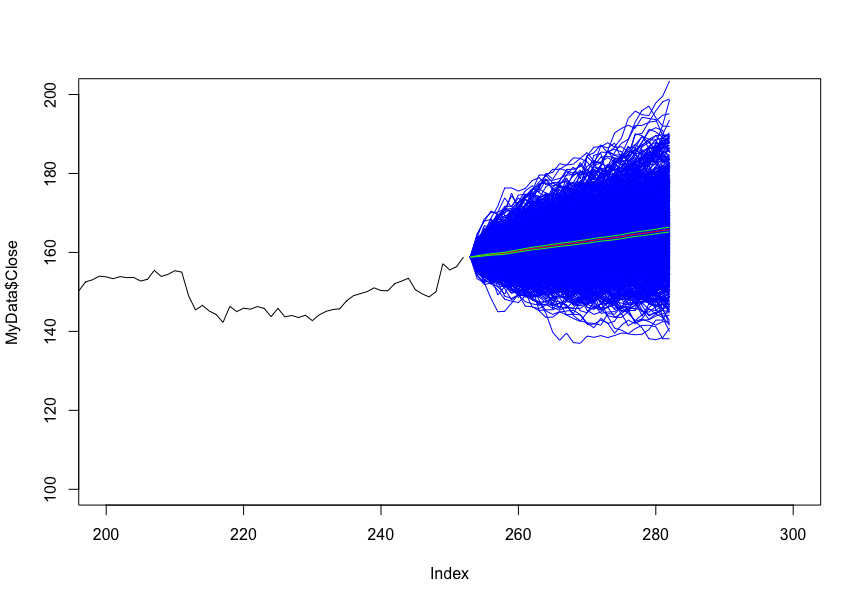
\includegraphics[width = \textwidth]{1000_trials_mean_error.png}
\\
The histogram below is the histogram of the distribution of the simulations of the stock price in 30 days. We can see that it is normally distributed. \\
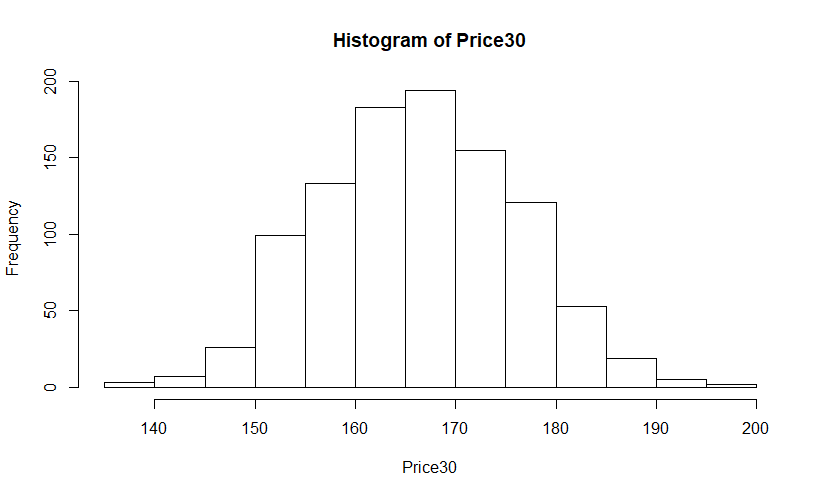
\includegraphics[width = \textwidth]{Rplot.png}\\
The table below shows the mean, variance, standard deviation, standard error and 95\% confidence interval of the mean of the stock price of Apple in 30 days: \\
\begin{table}[hbt]
  \centering
  \caption{Statistical Analysis}
  \label{stat}
  \begin{tabular}{|l|l|l|l|l|l|}
  \hline
  \multicolumn{1}{|c|}{} & Mean   & Variance & SD & SE & 95\% CI of mean\\ \hline
  Stock Price in 30 days & 166.31 & 94.41    & 9.72               & 0.60           & $\left(165.71, 166.91\right) $      \\ \hline
  \end{tabular}
\end{table}
\\
The table below shows the actual 68\%, 95\%, 99.7\% prediction interval for the price of the stock. Table one shows that the expected return is 166.31, but table two shows that there are chances that things could go crazy. For example, the stock price has 2.5\% of chance to hit lower than \$146.87 and 2.5\% of chance to be higher than \$185.75. 

\begin{table}[hbt]
\centering
\caption{Value at Risk}
\label{VaR}
\begin{tabular}{|l|l|l|l|}
\hline
\multicolumn{1}{|c|}{} & 68\%             & 95\%             & 99.7\%           \\ \hline
Value at Risk          & (156.59, 176.03) & (146.87, 185.75) & (137.15, 195.47) \\ \hline
\end{tabular}
\end{table}



\section{Results}


\subsection{Result}
In this project, we set the number of trials to be 1000 and we observe that the stock price of Apple is normally distributed. The expected value of the stock price is \$166.31. Since we have a big number of trials, we have a very low standard error for the mean, \$0.6, and it makes the 95\% confidence interval for the mean very narrow. However, when we look at the prediction interval of the stock prices, which is an estimate of an interval in which future observations will fall, in Table two, we observe some high risks.  The stock price of Apple has 16\% of chance to decrease \$9.72, 2.5\% of chance to decrease \$19.44 and 0.15\% of chance to decrease \$29.16. High risk is equivalent to high return. In the same time, investor has 16\% of chance to win \$9.72 on each share of stock, 2.5\% of chance to win \$19.44 on each share and 0.15\% of chance to win \$29.16 on each share. 


\subsection{Reasonableness}
Our result is reasonable as long as our assumption is solid, that there are no surprises in the market. We have a reasonable expected value for the stock price and the result also shows the high risk of the stock market. However, if the market or the company do meet some surprises, our prediction could be very bad. For example, a new employment policy or a new product could dramatically change the stock prices.

Meanwhile, the human behavior is also hard to model. In the real stock market, the stock price changes because of people buying in and selling out. When a big investment company tries to buy in or sell out some stock, this behavior can be infectious to other investors and would cause big changes to the price that our model would not be able to account for.

Additionally, people often expect the stock price to drop after a period time of increasing and even there is no sign in the market, people will start selling out because they are afraid of the ``upcoming drop”. What's more, we only generate the drift once in our model based on the historical data. In the real world, people can continuously update the data and compute the new drift after a time interval, and that can make the prediction more precise when making more immediate predictions.


\subsection{Validation}
We did a baseline comparison using our algorithm, but instead of predicting the stock price of next month, we simulate the price of this month. In the following plot, the black line is the actual price and the blue points are the simulated expected price for 30 days in this month. As the graph showing, our model gives a reasonable prediction about the trend of the future price. 

\includegraphics[width = \textwidth]{baseline1000.jpeg}

Additionally, we ran another baseline comparison using our algorithm comparing it to the entire previous year to see how the model did over a long term. The result produced both good and bad aspects. Our comparison showed that over the course of the year, the stock fluctuated a decent amount, while the mean of our monthly predictions did not and tended towards the larger of the two components, the drift. As a result of this, our model does not capture very accurately the price for any given day over the course of the predicted year. However, on the upside, we see that the final expected close price at the end of the year is still, in fact, quite close to the actual close price. This gives real evidence that our model is beneficial for long-term investors as it gives a solid idea of where the stock price might normally close in a year.

\section{Conclusions}

In conclusion, over the course of this research we developed an understanding for modeling stock prices. Through reading and examining existing literature and examples, we found several models and strategies for predicting the change in price of a stock after differing periods of time. Upon choosing a model, we simplified it into a mathematical model, clearly outlining our assumptions and the different components used, and adapted it for simulation and testing using Monte Carlo simulation. As a result of our algorithm we found a mean distributed prediction for which we were able to perform sensitivity analysis, helping us understand the accuracy and risk of this prediction. Lastly, we reviewed the resulting solution data and process for validity, showing that, while the model has both downsides and upsides, it is indeed a sound model that work for the particular problem.

Coming full circle, we arrive back at our original problem and the questions we sought to find answers for. Our final answer to the immediate problem is: yes, we can find a normally accurate and useful prediction for the closing price of a stock, such as Apple's stock, thirty days from the last known date, with the given assumption that there is no unexpected, dramatic volatility experienced over shorter intervals of prediction. Additionally, to our follow-up question of understanding risk involved with our prediction, we find a very appreciated result that we can get useful information for risk assessment purposes. Our model provides the statistical chance for both an upper and lower bound on the expected return from the stock.

Finally, through our research, we discovered many helpful insights and ideas which enables us to discuss the secondary questions we had about modeling stock price in general. To the question of "which model is best", we found it often varies, depending greatly on the specific environment for the stock and resulting data is desired. In attempting to augment our model, trying to make it more realistic, we found there is a wide range of possible events to account for. We described some of the previously in the results section, but things such as events, employee changes, stock selling/buying, and press releases all attribute possible changes of introducing their own shock to the stock's price. We weren't really able to find what events are more likely to effect a stock vs other events. In trying to profile chance of a certain type of event happening, we found it to be complex beyond anything would be reliable for the level of model we have. Multiple factors can cascade and cause massive, unexpected shock to the stock price, we were unable to find any model that accounted for the uncertainty of the future.

Through our research we learned a lot about how much models on the same topic can differ, simply by coming at the problem with a different approach. We also found that the initial choice in complexity of a model causes many consequences through using that model to study a topic. When the model is very complex, explaining and justifying it become very difficult, as well as analyzing the results. Lastly, we found that while at first glance a simpler model might have been less interesting, it ended up providing more stable results and reliable predictions of the stock price.

\pagebreak
\begin{thebibliography}{9}
\bibitem{ApplicationGBM}
Simulating Stock Prices Using Geometric Brownian Motion: Evidence from Australian
Companies
\bibitem{MathFinMarkets}
Can Math Beat Financial Markets?
\bibitem{WikiBModel}
Wikipedia: Brownian Model of Financial Markets\\
\texttt{https://en.wikipedia.org/wiki/Brownian-model-of-financial-markets}
\bibitem{RW}
Random Walk Theory\\
\texttt{http://www.investopedia.com/terms/r/randomwalktheory.asp}
\bibitem{WikiBSModel}
Wikipedia: Black-Scholes Model\\
\texttt{https://en.wikipedia.org/wiki/Black-Scholes-model\# Short-stock-rate}
\bibitem{GBMoverBM}
Geometric Brownian Motion
\texttt{http://www.columbia.edu/\~ ks20/FE-Notes/4700-07-Notes-GBM.pdf}
\bibitem{GBM}
Geometric Brownian Motion\\
\texttt{http://www.math.uah.edu/stat/brown/Geometric.html}
\bibitem{GFSandANN}
Integration of genetic fuzzy systems and artificial neural networks for stock price forecasting
\end{thebibliography}



	
	
	
\end{document}
